\documentclass[10pt]{beamer}

%packages
\usepackage{babel}
\usepackage[utf8]{inputenc}
\usepackage{amsmath,tabu}
\usepackage{color}
\usepackage{tikz}
\usetikzlibrary{matrix,chains,positioning,decorations.pathreplacing,arrows}
\usetikzlibrary{fit,shapes}
\usetikzlibrary{calc,shadings}
\usepackage{pgfplots}
\usepackage{colortbl}
\usepackage{eurosym}
\usepackage{mathtools}
\usepackage{listings}
\usepackage{tabularx}

%definitions
\usepackage{algorithm,algorithmic}

%theme
\usetheme{Dresden}
\usecolortheme{rose}
\useoutertheme{tree}

%environments
\newenvironment{ExampleGer}{\begin{exampleblock}{Beispiel}}{\end{exampleblock}}

\newenvironment{customlegend}[1][]{%
	\begingroup
	% inits/clears the lists (which might be populated from previous
	% axes):
	\csname pgfplots@init@cleared@structures\endcsname
	\pgfplotsset{#1}%
}{%
	% draws the legend:
	\csname pgfplots@createlegend\endcsname
	\endgroup
}%

%definitions
\def\addlegendimage{\csname pgfplots@addlegendimage\endcsname}
% definition to insert numbers
\pgfkeys{/pgfplots/number in legend/.style={%
		/pgfplots/legend image code/.code={%
			\node at (0.295,-0.0225){#1};
		},%
	},
}

%general
\title{Combining bottom up and top down approaches for Drug-Target-Interaction prediction}
\author{Tilman Hinnerichs}
\institute{BORG - KAUST}
\date{December 09, 2019}

%presentation
\expandafter\def\expandafter\insertshorttitle\expandafter{%
	\insertshorttitle\hspace{5cm}%
	\insertframenumber\,/\,\inserttotalframenumber
}

\definecolor{myblue}{RGB}{80,80,160}
\definecolor{mygreen}{RGB}{80,160,80}
\definecolor{myturk}{RGB}{240,60,60}

\begin{document}
	
\begin{frame}
	\titlepage
\end{frame}

\begin{frame}{Outline}
	\setbeamertemplate{section in toc}[sections numbered]
	\tableofcontents
\end{frame}

\section{Problem Description}
\begin{frame}{Problem Description}
	Prediction over bipartite graph:
	
	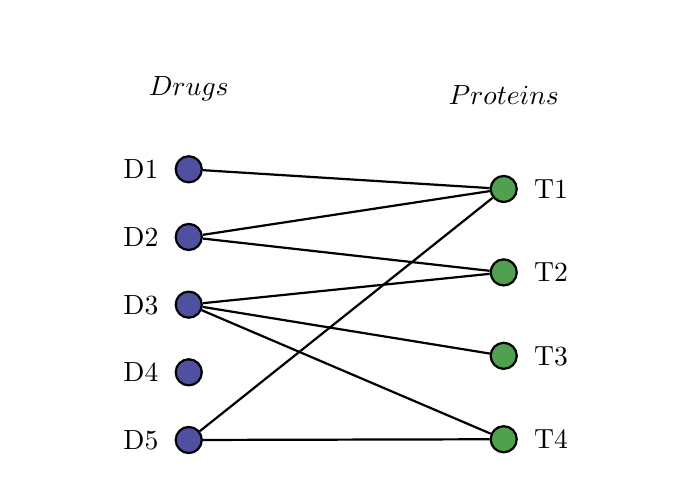
\begin{tikzpicture}[thick,
	every node/.style={draw,circle},
	fsnode/.style={fill=myblue},
	fs1node/.style={fill=myblue},
	ssnode/.style={fill=mygreen},
	%every fit/.style={ellipse,draw,inner sep=-1pt,text width=2cm},
	%->,shorten >= 3pt,shorten <= 3pt
	]
	
	% the vertices of U
	\begin{scope}[start chain=going below,node distance=5mm]
	\foreach \i in {1,2,...,3}
	\node[fsnode,on chain] (f\i) [label=left: D\i] {};
	\end{scope}
	
	% the vertices of U1
	\begin{scope}[node distance=5mm]
	\foreach \i in {4,5}
	\node[fs1node,on chain] (f\i) [label=left: D\i] {};
	\end{scope}
	
	% the vertices of V
	\begin{scope}[xshift=4cm,yshift=-0.25cm,start chain=going below,node distance=7mm]
	\foreach \i in {1,2,...,4}
	\node[ssnode,on chain] (s\i) [label=right: T\i] {};
	\end{scope}
	
	% the set U
	%\node [myblue, fit=(f1) (f3)] {};
	\node [white,fit=(f1) (f5),label=above:$Drugs$] {};
	
	% the set V
	\node [white,fit=(s1) (s4),label=above:$Proteins$] {};
	
	% the edges
	\draw (f1) -- (s1);
	\draw (s1) -- (f2);
	\draw (f2) -- (s2);
	\draw (s2) -- (f3);
	\draw (s3) -- (f3);
	\draw (f3) -- (s4);
	\draw (s4) -- (f5);
	\draw (f5) -- (s1);
	\end{tikzpicture}
	
\end{frame}

\section{Recent approaches}
\begin{frame}{Classification of recent approaches\footnote{Chen Wang et al., Briefings in Bioinformatics, 2018}\footnote{Yu Ding et al., Briefings in Bioinformatics, 2019}}
	\begin{table}
		\begin{tabularx}{\textwidth}{|>{\setlength\hsize{.5\hsize}\setlength\linewidth{\hsize}}X|>{\setlength\hsize{1.25\hsize}\setlength\linewidth{\hsize}}X|>{\setlength\hsize{1.25\hsize}\setlength\linewidth{\hsize}}X|}
			\hline
			&Drugs&Protein\\
			\hline
			bottom-up&
			\begin{itemize}
				\item GCN over molecules
				\item drug similarity
			\end{itemize}&
			\begin{itemize}
				\item secondary structure prediction
				\item contact prediction
				\item convolution over amino acid sequences
			\end{itemize}\\
			\hline
			top-down&
			\begin{itemize}
				\item network approaches
				\item drug similarity
			\end{itemize}&
			\begin{itemize}
				\item protein similarity
			\end{itemize}\\
			\hline
		\end{tabularx}
	\end{table}	
\end{frame}

\begin{frame}{Problems of recent approaches}
	Main issues:
	\begin{itemize}
		\item Lack ability to generalize or are unable to spot small differences
		\item Usually only top-down or bottom-up
		\item Not making use of interaction networks
	\end{itemize}
	\pause
	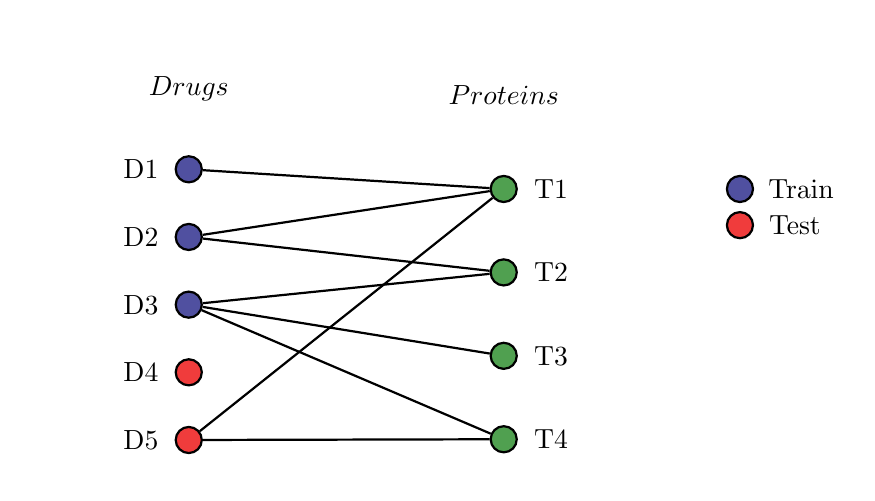
\begin{tikzpicture}[thick,
	every node/.style={draw,circle},
	fsnode/.style={fill=myblue},
	fs1node/.style={fill=myturk},
	trainlegendnode/.style={fill=myblue},
	testlegendnode/.style={fill=myturk},
	ssnode/.style={fill=mygreen},
	%every fit/.style={ellipse,draw,inner sep=-1pt,text width=2cm},
	%->,shorten >= 3pt,shorten <= 3pt
	]
	
	% the vertices of U
	\begin{scope}[start chain=going below,node distance=5mm]
	\foreach \i in {1,2,...,3}
	\node[fsnode,on chain] (f\i) [label=left: D\i] {};
	\end{scope}
	
	% the vertices of U1
	\begin{scope}[node distance=5mm]
	\foreach \i in {4,5}
	\node[fs1node,on chain] (f\i) [label=left: D\i] {};
	\end{scope}
	
	% the vertices of V
	\begin{scope}[xshift=4cm,yshift=-0.25cm,start chain=going below,node distance=7mm]
	\foreach \i in {1,2,...,4}
	\node[ssnode,on chain] (s\i) [label=right: T\i] {};
	\end{scope}
	
	% legend
	\begin{scope}[xshift=7cm,yshift=-0.25cm,start chain=going below,node distance=7mm]
	\foreach \i in {1}
	\node[trainlegendnode,on chain] (trainlegend\i) [label=right: Train] {};
	\end{scope}
	
	\begin{scope}[xshift=7cm,yshift=-0.25cm, node distance=1mm]
	\foreach \i in {1}
	\node[testlegendnode,on chain] (testlegend\i) [label=right: Test] {};
	\end{scope}
	
	% the set U
	%\node [myblue, fit=(f1) (f3)] {};
	\node [white,fit=(f1) (f5),label=above:$Drugs$] {};
	
	% the set V
	\node [white,fit=(s1) (s4),label=above:$Proteins$] {};
	
	% the edges
	\draw (f1) -- (s1);
	\draw (s1) -- (f2);
	\draw (f2) -- (s2);
	\draw (s2) -- (f3);
	\draw (s3) -- (f3);
	\draw (f3) -- (s4);
	\draw (s4) -- (f5);
	\draw (f5) -- (s1);
	\end{tikzpicture}
	
\end{frame}

\section{A medium approach to DTI prediction}
\begin{frame}{How to bring both approaches together?}
	\begin{enumerate}
		\item For each drug, filter possible targets according to protein based measurement
		\item Bring those together with the interaction networks for the prediction
	\end{enumerate}
\end{frame}

\subsection{Filtering possible targets}
\begin{frame}{How to build such a filter?}
	STITCH database got 
	\begin{itemize}
		\item 390 000 chemicals, and
		\item 3.6 million proteins
		\item from over 2000 organisms
	\end{itemize}
	\pause 
	\vspace{0.5cm}
	For each drug, find a motif in the target amino acid sequences and query that against all possible proteins and use the results as features for the prediction
\end{frame}

\begin{frame}{How to find motifs?}
	\begin{enumerate}
		\item Build multi sequence alignment with alignment tool of choice over non-human proteins
			\begin{itemize}
				\item FAMSA, MAFFT, Kalign, MSA Props, Muscle, \dots
			\end{itemize}
		\item Build representation of that alignment
			\begin{itemize}
				\item Hidden Markov model with HMMER
				\item PWM
			\end{itemize}
		\item Query representation against database
	\end{enumerate}
	\pause
	\vspace{0.5cm}
	This is very expensive to compute \dots (10000 hours for alignments of 614 drugs + IBEX queue times for such big jobs)
\end{frame}

\begin{frame}{}
\end{frame}


\begin{frame}{Full citations}
	\footnotesize
	\begin{itemize}
		\item Yu Ding, Hong Wang, Hewei Zheng, Lianzong Wang, Guosi Zhang, Jiaxin Yang, Xiaoyan Lu, Yu Bai, Haotian Zhang, Jing Li, Wenyan Gao, Fukun Chen, Shui Hu, Jingqi Wu, Liangde Xu, Evaluation of drug efficacy based on the spatial position comparison of drug–target interaction centers, Briefings in Bioinformatics, , bbz024, https://doi.org/10.1093/bib/bbz024
		\item Chen Wang, Lukasz Kurgan, Review and comparative assessment of similarity-based methods for prediction of drug–protein interactions in the druggable human proteome, Briefings in Bioinformatics, , bby069, https://doi.org/10.1093/bib/bby069
	\end{itemize}
\end{frame}


\end{document}